\section{Competition results: baselines and notable approaches}
\label{sec:results}

The competition received a total of 26 entries.
%
This section summarizes the competition results for each track,
and discusses the techniques used by the track winners and the baselines.
%
The state of the framework and the results, post competition, are captured on Github in 
\href{https://github.com/harsha-simhadri/big-ann-benchmarks/releases/tag/v0.3.0}{v0.3}.

\subsection{Filtered Search Track}

The organizers provided a baseline implementation \texttt{faiss} of the filtered search track based on Faiss~\cite{douze2024faiss}. 
The baseline operates in two possible modes. 
In vector-first mode, the search is performed with a Faiss IVF index and vector results that do not satisfy the tag constraint are removed from the result list. 
In metadata-first mode, the database is reduced to the vectors satisfying the word constraint; in that case the vector search is performed brute force. 
See \cite[Section 6.2]{douze2024faiss} for more details. 
The baseline is reasonably optimized but uses vanilla Faiss, with parts implemented in Python. 


% \begin{figure}[t!]
% \hspace*{-2em}
% \begin{minipage}[b]{0.65\textwidth}
%         \centering
% 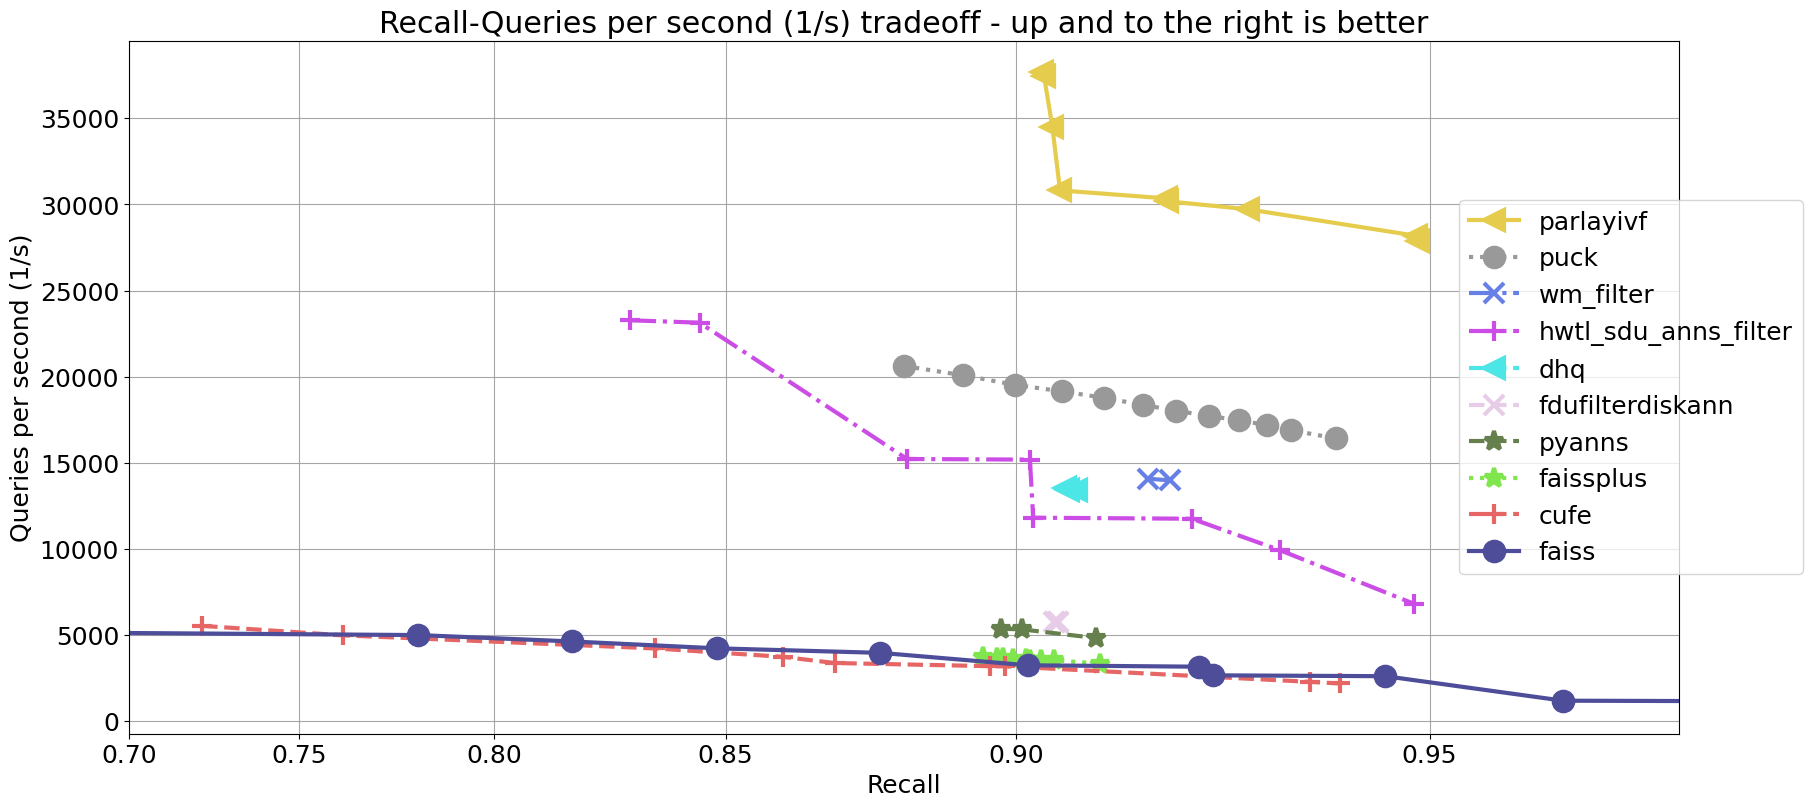
\includegraphics[width=\textwidth]{fig/yfcc-10M.png}
%     \captionof{figure}{Performance of the different algorithms in the filter track on the private query set.}
%     \label{fig:filter_results}
% \end{minipage}    
% ~
% \begin{minipage}[b]{0.38\textwidth}
% \centering
% \begin{tabular}{lrr}
% %\hline
% Algorithm             & QPS       & QPS \\
%                       & (private) & (public) \\
% %\hline
% parlayivf             & 37671     & 37902 \\
% puck                  & 19153     & 19193 \\
% hwtl\_sdu\_anns\_filter  & 15189     & 15059 \\
% wm\_filter             & 14076     & 14468 \\
% dhq                   & 13517     & 13671 \\
% fdufilterdiskann      & 5752      & 5680  \\
% pyanns                & 5336      & 5185  \\
% faissplus             & 3625      & 3777  \\
% faiss                 & 3253      & 3033  \\
% cufe                  & 2291      & 2917 \\
% %\hline
% \end{tabular}
% \captionof{table}{Highest QPS achieved by any algorithm in the filtered track (private and public query sets), as long as the recall@10 is at least 0.9.}\label{tab:filter}
% \end{minipage}
% \end{figure}

\begin{figure*}[t!]
        \centering
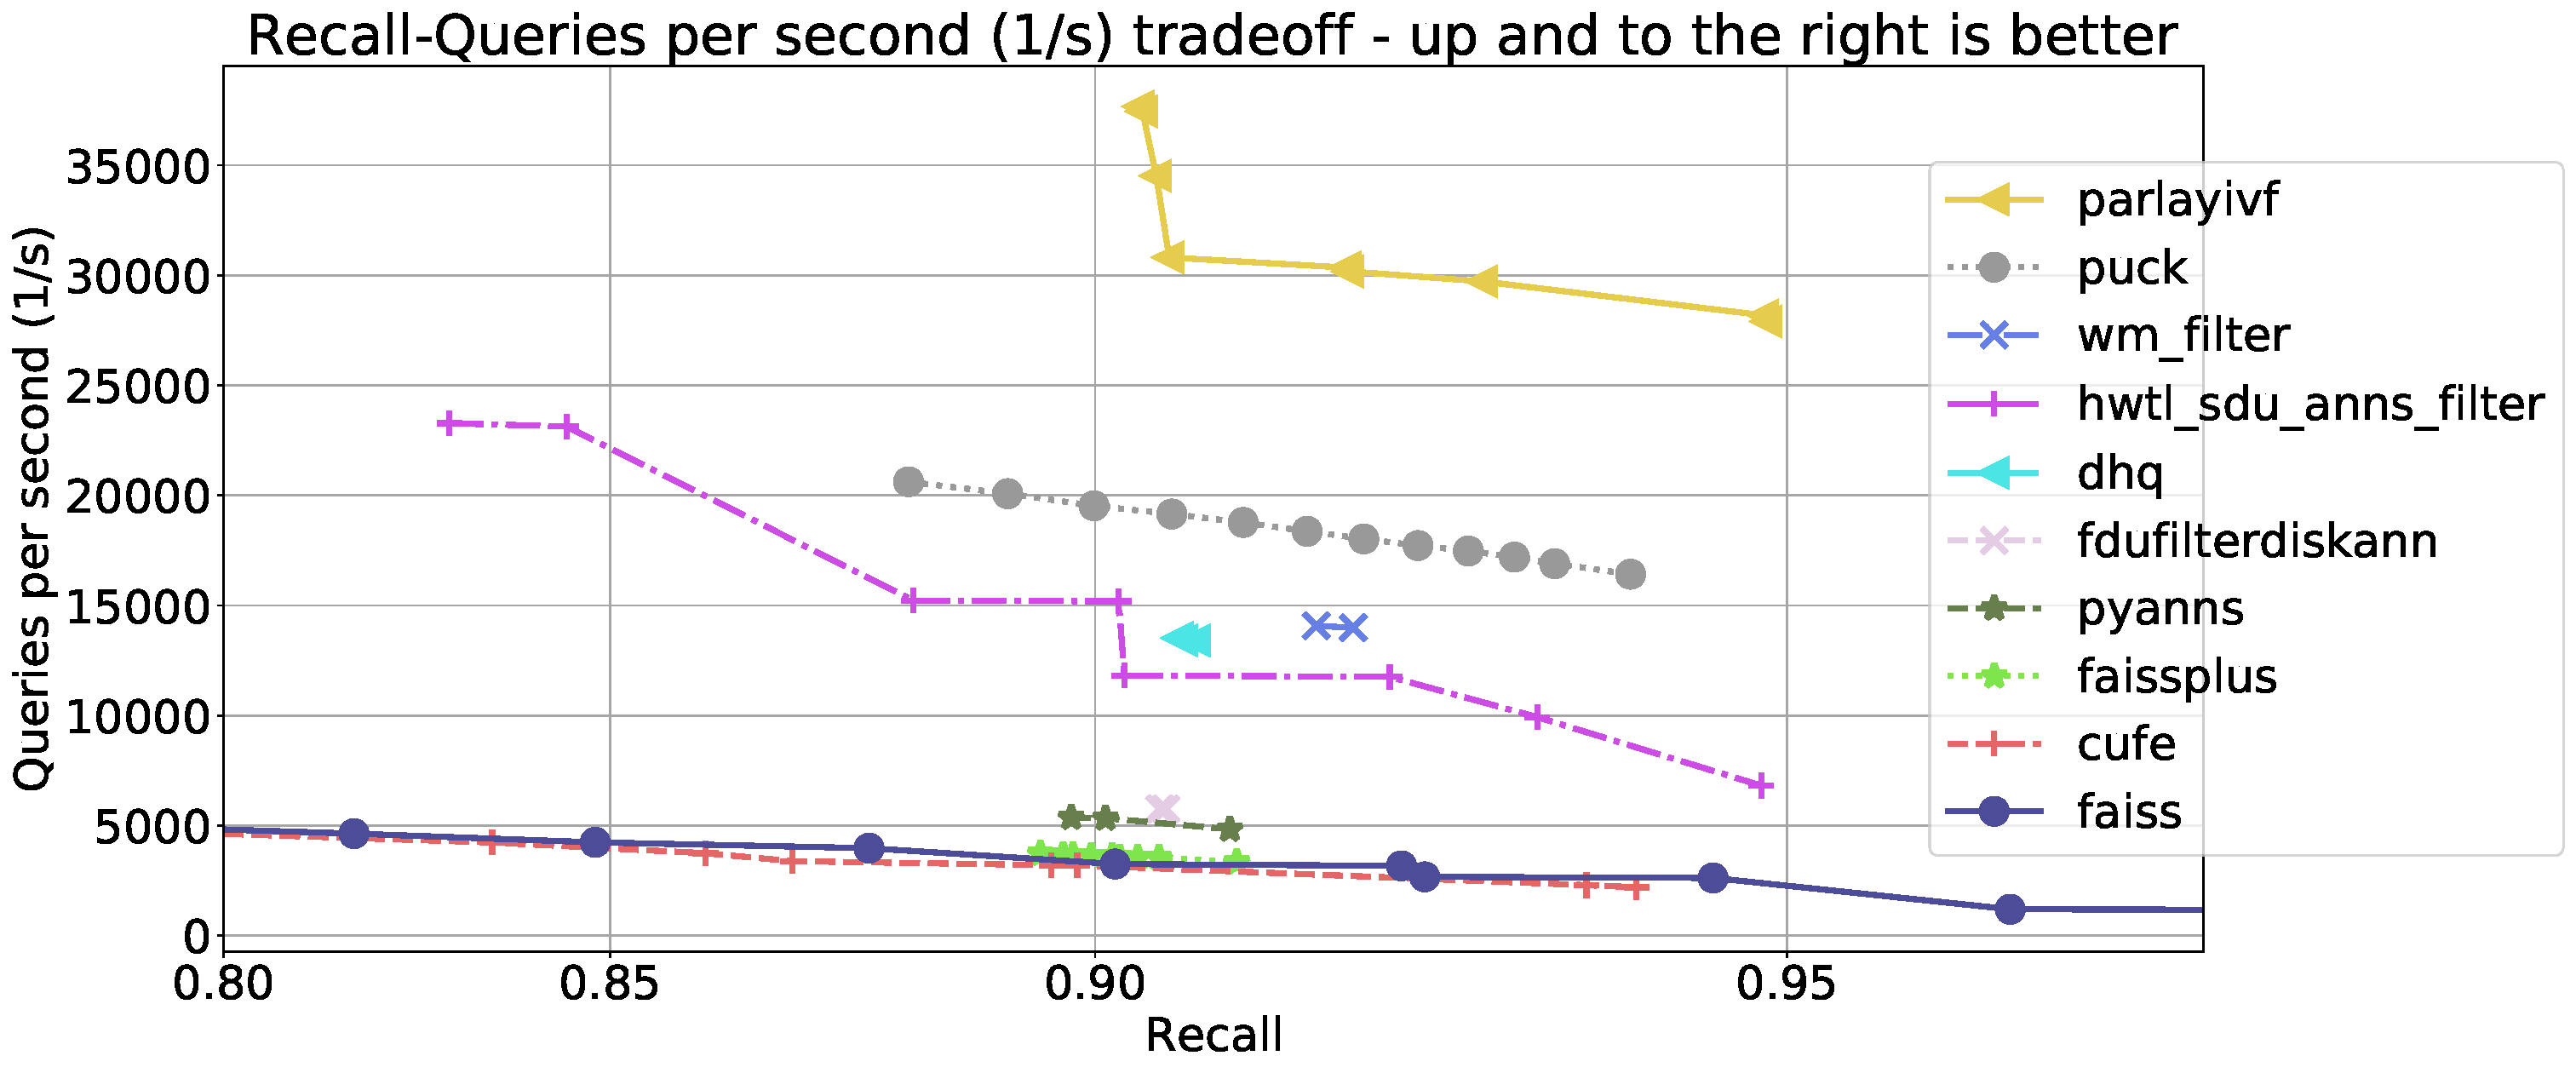
\includegraphics[width=.75\textwidth]{fig/yfcc-10M-2.pdf}
    \captionof{figure}{Performance of the different algorithms in the filtered track on the private query set.}
    \label{fig:filter_results}
    \ifnotarxiv
    \vspace*{-10pt}
    \fi
\end{figure*}

\begin{table*}[t!]
\small
\centering
\begin{tabular}{lrrrrrrrrrr}
\hline
\textbf{Algorithm}     & parlay & puck  & hwtl & wm & dhq   & fdu & pyanns & faiss+ & faiss & cufe \\ \hline
\textbf{QPS (pub)}  & 37902     & 19193 & 15059                   & 14468      & 13671 & 5680             & 5185   & 3777      & 3033  & 2917 \\
\textbf{QPS (priv)} & 37671     & 19153 & 15189                   & 14076      & 13517 & 5752             & 5336   & 3625      & 3253  & 2291 \\ \hline
\end{tabular}
\caption{Highest QPS achieved by any algorithm in the filtered track with public (pub) and private (priv) query sets, as long as the recall@10 is at least 0.9. Entry names are abbreviated.}
\label{tab:filter}
\ifnotarxiv
\vspace*{-20pt}
\fi
\end{table*}

We received ten submissions. 
Fig.~\ref{fig:filter_results} and Table~\ref{tab:filter} summarize the results of the different algorithms on the Filtered track.
The top result is more than 11x faster than the baseline implementation. We observe that there are no major discrepancies between the performance on the public and the private query workload. 
The participants chose to vary their 10 search hyperparameters to different degrees; all provided usually more than one parameter setting exceeding the target recall.

The winning team ParlayANN (\texttt{parlayivf}) used an index whose primary key is the tag associated to each database item. 
For common tags that are shared by many vectors, a Vamana~\cite{DiskANN19} graph as well as a spatial inverted index are constructed to index them, less common tags are just stored sequentially. 
At search time, for single-tag queries, the relevant subset of the dataset is accessed immediately and searched, using either a Vamana graph or linear scan. 
For two-tag queries, three different strategies are used. If one tag corresponds to a set of low cardinality and the other to a set of high cardinality, the smallest tag's elements are intersected with a subset of the largest ones using an efficient bit vector. If both tags correspond to sets of high cardinality, the corresponding spatial indices are used to generate a list of candidates for each tag, and then the intersection of those two candidates is returned. If both tags correspond to sets of low cardinality, the intersection is computed linearly.
The queries are ordered to perform similar queries in sequence to improve the cache behavior. 

%\magdalen{The paragraph below doesn't seem to belong here--we should probably remove}
%\matthijs{What makes you think that? This describes the Baidu submission}
The second-place submission from Baidu (\texttt{puck}) is implemented in the Puck library (\url{https://github.com/baidu/puck}). 
The index structure has four filtering levels. 
The first two levels are trained using vector quantization, the last two ones employ product quantization.
Each cluster in the levels is labelled with the tags of the vectors in that cluster. 
This allows to filter out centroids at search time based on the tags.%, handled with a callback similar to the baseline implementation. 

As visible from the description, the excellent performance of the top participants of this track comes from genuinely handling the filtering constraints with more appropriate data structures.  
The search for better hyperparameters on the baseline only resulted in minor differences, as visible in the difference between \texttt{faiss}, \texttt{faissplus}, and \texttt{cufe}.

%the tag of a centroid is a collection of points’ labels in this centroid.
%for each query, centroids that do not meet the requirements are filtered.
%For the first pq level, points that do not meet the requirements are filtered. filtering is implemented via a callback similar to the baseline implementation. Keep the top-M most similar samples as the candidate set.
%For the second pq level, Re-rank samples in the candidate set and return top-K.

\ifnotarxiv

\begin{figure*}[t]
\begin{minipage}[b]{0.7\textwidth}
\centering
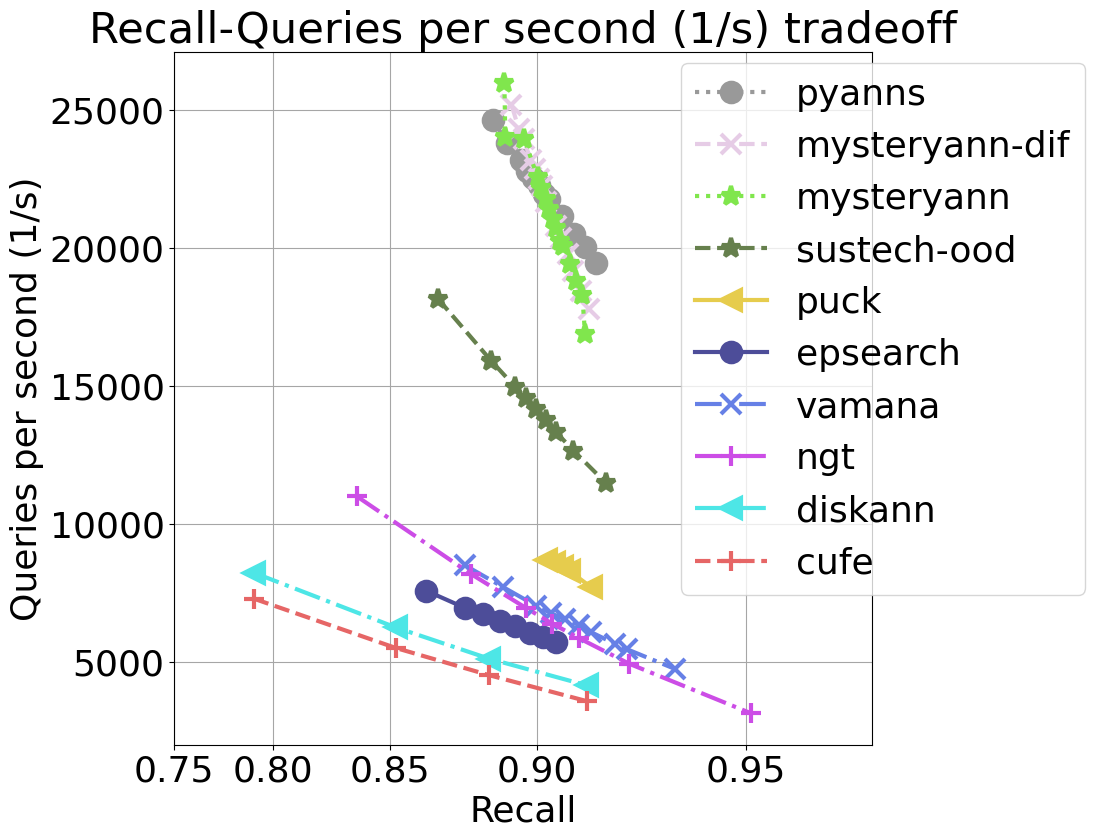
\includegraphics[width=0.6\textwidth]{fig/text2image-10M.png}
    \captionof{figure}{Performance of the different algorithms in the OOD track.}
    \label{fig:ood_results}    
\end{minipage}
~
\begin{minipage}[b]{0.28\textwidth}
\centering
\small
\begin{tabular}{lrr}
\hline
Algorithm & QPS \\
\hline
pyanns &  22296 \\
mysteryann-dif & 22492 \\
sustech-ood  & 13772\\
puck & 8700 \\ 
vamana & 6753 \\
ngt &  6374 \\
epsearch & 5877 \\
cufe &  3561 \\
\hline
\end{tabular}
\captionof{table}{Highest QPS achieved by any algorithm in the OOD track, as long as the recall@10 is at least 0.9.}\label{tab:ood}
\end{minipage}
\end{figure*}

\fi 

%%%%%%%%%%%%%%%%%% version for ArXiV

\ifarxiv

\begin{figure}
\centering
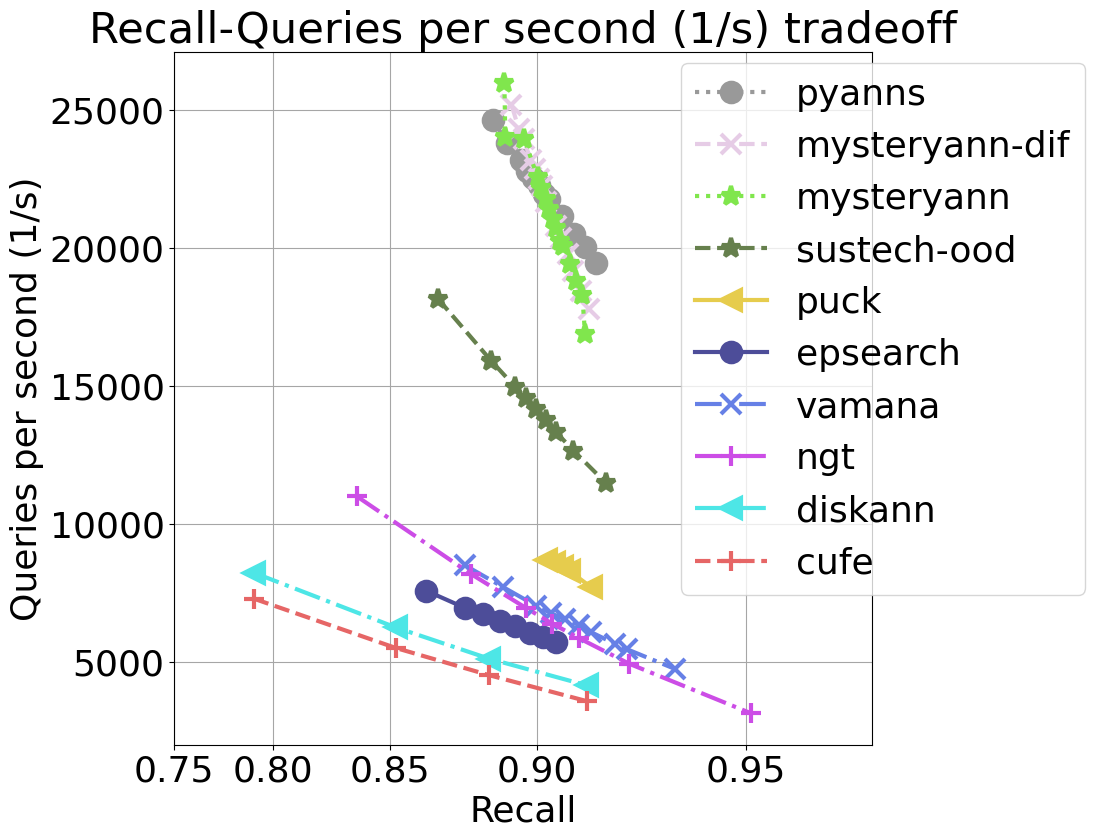
\includegraphics[width=0.9\linewidth]{fig/text2image-10M.png}
    \caption{Performance of the different algorithms in the OOD track.}
    \label{fig:ood_results}    
\end{figure}

\begin{table}
\centering
\begin{tabular}{lrr}
\hline
Algorithm & QPS \\
\hline
pyanns &  22296 \\
mysteryann-dif & 22492 \\
sustech-ood  & 13772\\
puck & 8700 \\ 
vamana & 6753 \\
ngt &  6374 \\
epsearch & 5877 \\
cufe &  3561 \\
\hline
\end{tabular}
\caption{Highest QPS achieved by any algorithm in the OOD track, as long as the recall@10 is at least 0.9.}\label{tab:ood}
\end{table}

\fi 

\subsection{Out-Of-Distribution (OOD) Track}
The baseline for the OOD track was the in-memory index variant \texttt{vamana} in the DiskANN library~\cite{Diskann-v0.5}. 
%
While a variant of DiskANN adapted to query distributed exists~\cite{jaiswal2022ooddiskann},
the baseline does not use those ideas and %, and is not adapted to the query distribution.
%
uses only the points in the database to construct the index.
%


This track had eight submissions. Fig.~\ref{fig:ood_results} and Table~\ref{tab:ood} show the results of the different algorithms  (this track only had a public query set). Due to extremely close performance, MysteryANN (later renamed RoarANN) and PyANNS were declared the joint winners of the track. 

RoarANN adopted a graph-based approach, with performance accelerated by scalar quantization and graph reordering. Their graph-based approach took the query vector distribution into account by initially building a bipartite graph between the base distribution and a sample from the query distribution, where each query sample received a directed edge from its top nearest neighbor in the base distribution, and sent $k-1$ directed edges to its remaining $k$ nearest neighbors in the base distribution. The graph was then projected back into the base distribution. After computing these query-based edges, additional edges were computed using the standard procedure for ANNS graph algorithms in order to form a connected and searchable graph. The approach is published in ~\cite{DBLP:journals/pvldb/ChenZHJW24}.

PyANNS also used a graph-based approach but did not specifically adapt its algorithm for the out-of-distribution setting. It achieved its winning QPS through careful engineering and optimization of its core library. It used a Vamana graph with a standard greedy search. The search used a scalar quantization of the vectors to 8 bits, with reranking using a 16-bit scalar quantization. The author credits the strong performance of PyANNS to the aforementioned quantization, use of Vector Neural Network Instructions (VNNI), and an adaptive prefetching strategy. 

The results show that improvements over the baseline could be achieved in two ways: Through careful algorithm design that adapts the index to the setting of out-of-distribution queries (RoarANN), and through careful implementation engineering (PyANNS).



\subsection{Sparse Track}
The baseline for this track was  the \texttt{linscan} algorithm~\cite{bruch2023approximate} available in~\cite{Linscan-github},
which is based on an efficient linear scan of an inverted index. 
%
Search was accelerated by considering only the largest elements of the query vector,
at the expense of accuracy.
%


We received five submissions each of which used a different technique. 
Their performance in terms of recall-QPS is shown in Fig.\ref{fig:sparse_results} and their highest throughput above recall .9 can be found in Table~\ref{tab:sparse}. 

%%%%%%%%%% for neurips: 
\ifnotarxiv
\begin{minipage}{\textwidth}
\begin{minipage}[b]{0.6\textwidth}
    \centering
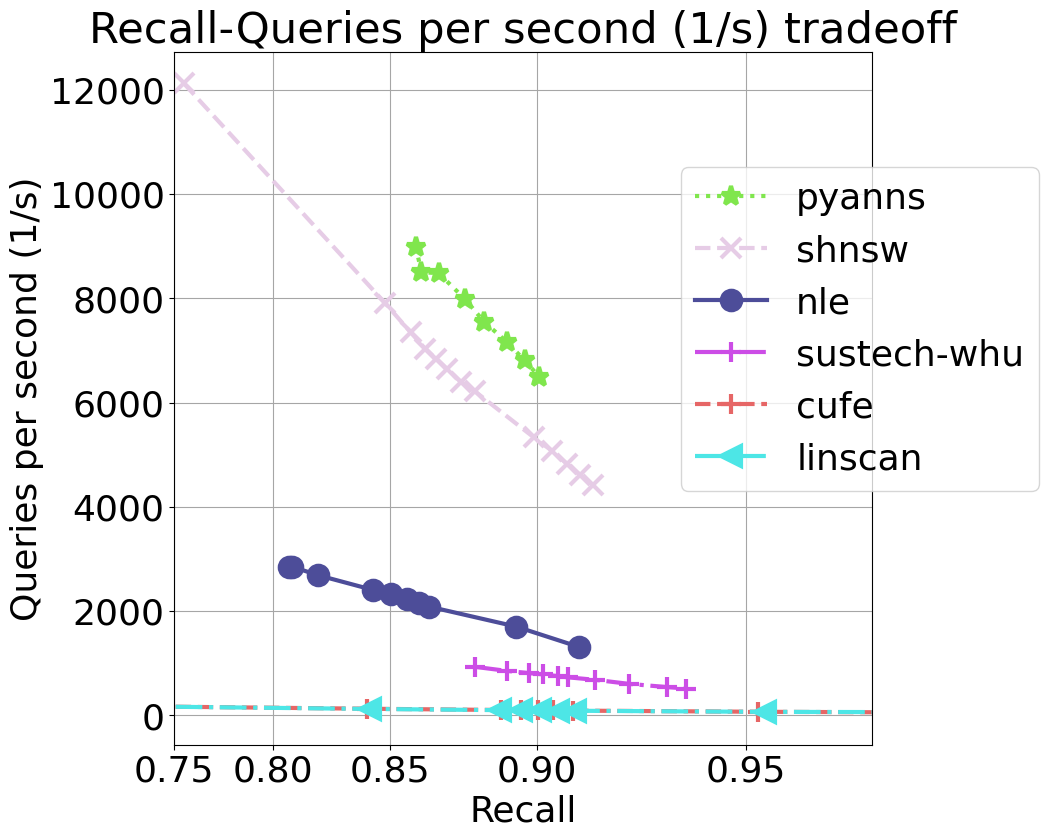
\includegraphics[width=.6\textwidth]{fig/sparse-full.png}
    \captionof{figure}{Performance of the different algorithms in the sparse track on the private query set.}
    \label{fig:sparse_results}
\end{minipage}
~
\begin{minipage}[b]{0.38\textwidth}
\centering
\small
\begin{tabular}{lrr}
\hline
Algorithm & QPS       & QPS \\
          & (private) & (public) \\
\hline
pyanns & 6500 & 8732 \\
shnsw & 5078 & 7137 \\
nle & 1313 & 2359 \\
sustech-whu & 788 & 1015\\ 
cufe & 98 & 105 \\
linscan & 95 & 93 \\
\hline
\end{tabular}
\captionof{table}{Highest QPS achieved by any algorithm in the sparse track (private and public query sets), as long as the recall@10 is at least 0.9.}\label{tab:sparse}
\end{minipage}
\end{minipage}
\fi 

%%%%%%%% for ArXiV: regular figures 
\ifarxiv 

\begin{figure}
    \centering
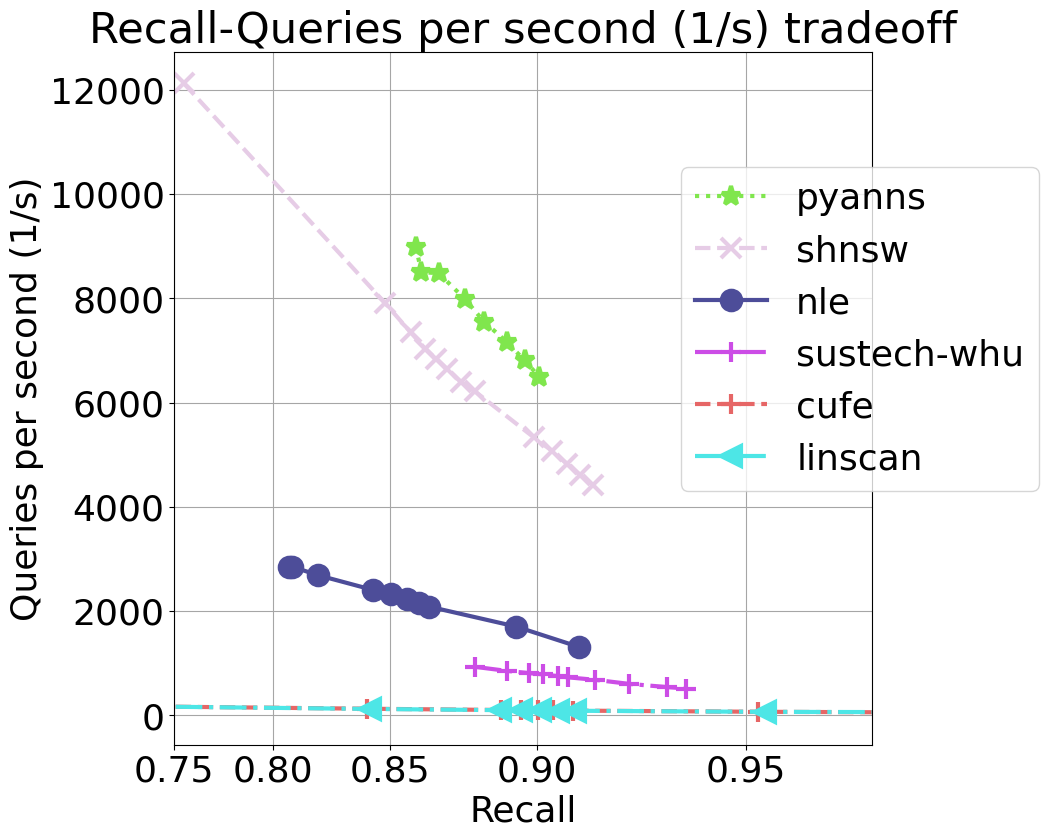
\includegraphics[width=.9\linewidth]{fig/sparse-full.png}
    \caption{Performance of the different algorithms in the sparse track on the private query set.}
    \label{fig:sparse_results}
\end{figure}

\begin{table}
\centering
\begin{tabular}{lrr}
\hline
Algorithm & QPS       & QPS \\
          & (private) & (public) \\
\hline
pyanns & 6500 & 8732 \\
shnsw & 5078 & 7137 \\
nle & 1313 & 2359 \\
sustech-whu & 788 & 1015\\ 
cufe & 98 & 105 \\
linscan & 95 & 93 \\
\hline
\end{tabular}
\captionof{table}{Highest QPS achieved by any algorithm in the sparse track (private and public query sets), as long as the recall@10 is at least 0.9.}\label{tab:sparse}
\end{table}

\fi 

\ifarxiv
The winners of the sparse track are:
\begin{description}
   \item[PyANNS,]by Zihao Wang, Shanghai Jiao Tong University\footnote{Zihao Wang is also an employee of Zilliz.
   However, he declares that the PyANNs entry was created on his time off, without any involvement from Zilliz or any of the other organizers.
   This entry did not declare conflict with organizers before participating.}.
   \item[GrassRMA:] GRAph-based Sparse Vector Search with Reducing Memory Accesses, by Meng Chen, Yue Chen, Rui Ma, Kai Zhang, Yuzheng Cai, Jiayang Shi, Yizhuo Chen, Weiguo Zheng. All authors from Fudan University\footnote{GrassRMA was previously called \textbf{shnsw}}.
\end{description}
\fi

The winning submissions, PyANNS (\texttt{pyanns}) and GrassRMA (\texttt{shnsw}), both used an HNSW-based graph index~\cite{HNSW16} but applied different optimizations.
%The optimizations employed by PyANNS are as follows.
PyANNS quantized vector coordinates to 16 bit integers and vector values to 16 bit half-precision floats.
Further, during the graph search, the coordinates of vectors in the database were represented as 8-bit integers,
and smaller values of the query were pruned away.
In order to recover from the accuracy degradation due to the quantization and pruning,
the graph search was followed by a refinement step using the full query vector and
higher precision base vectors.  GrassRMA employed the following optimizations: 
(1) co-locating coordinates and values of  the vector to  improve memory access, and 
(2) keeping an upper and lower bound of the values in the vectors in the index
in order to early terminate the dot product calculation.%\footnote{It is an interesting open question whether a solution incorporating the memory access patterns of GrassRMA and the reduced precision and caching of PyANNs would result in an even better performing algorithm.}
Summarizing the winning submissions, they won through careful engineering of existing baselines. 

\ifarxiv
These were the other submissions in the sparse track. 
%
The NLE team used a fast text search engine (pisa\cite{mallia2019pisa}), and modified it in order to support general sparse vectors.
%
sustech-whu is also based on hnsw, in a manner that turned out to be less efficient then the other graph submissions.
%
The submission cufe is a minor modification of the baseline algorithm, linscan\cite{bruch2023approximate}. 

\fi

We also note the performance differences between the public and private queries.
%
Several algorithms (pyanns,  shnsw, sustech-whu) performed around 25\% slower on private queries,
while nle performed significantly worse (around 45\% slower), showing potentially over-fitting on the public queries.
%
\ifarxiv
In terms of index build time, all submissions were able to successfully build an index within the alotted 12 hour limit,
with the exception of sustech-whu, that needed 14 hours to build the index.
\fi

\subsection{Streaming Search Track}

The baseline for this track was the streaming in-memory index variant \texttt{diskann} from the DiskANN library\cite{Diskann-v0.5} using ideas described in~\cite{FreshDiskaNN}.
%
%The index uses the insertion and graph clean up ideas described in the FreshDiskANN paper~\cite{FreshDiskaNN}.
%
While point insertions are processed eagerly, deletions are processed lazily. 
% 
A deletion vector is marked as such immediately, but the graph surrounding is not immediately cleaned up.
%
%Accumulating a large number of deletes leads to a drop in index recall, normalizing for search parameters.
%
When the index is close to running out of space for inserting new vectors, it runs a "consolidation" method
that frees up deleted vectors and re-organizes the graph around deleted nodes to improve search quality.
%
%Consolidation improves the recall of the graph index. 
%
A more detailed analysis of the recall trends of the baseline and HNSW algorithms is provided in the \href{https://github.com/harsha-simhadri/big-ann-benchmarks/blob/v0.3/neurips23/notes/streaming/hnsw\_result/hnsw\_result.md}{framework}.
%\footnote{
%\url{https://github.com/harsha-simhadri/big-ann-benchmarks/blob/v0.3/neurips23/notes/streaming/hnsw\_result/hnsw\_result.md}}

The streaming track received four entries in total.
%
The entrants were judged by their average recall for queries over the entire runbook, with an hour time limit for executing the runbook, and the official competition results can be found in Table~\ref{tab:streaming_competition}. 

\begin{table*}[ht]
\small
\begin{minipage}{0.38\textwidth}
\begin{tabular}{lrr}
\hline
Algorithm & Recall \\
\hline
puck &  0.985\\
hwtl\_sdu\_anns\_stream &  0.9674\\
pyanns &  0.9597 \\
diskann & 0.883 \\
cufe & 0.8189 \\ 
\hline
\end{tabular}
\caption{Recall reported for entries in the official results for the streaming track.}\label{tab:streaming_competition}
\end{minipage}\centering
~~~~~~~~
\begin{minipage}{0.38\textwidth}
\centering
\begin{tabular}{lrr}
\hline
Algorithm & Recall \\
\hline
pyanns & 0.8865 \\
hwtl\_sdu\_anns\_stream & 0.7693 \\
diskann & 0.7218 \\
cufe & 0.6481  \\
puck & 0.0921 \\ 
\hline
\end{tabular}
\caption{Recall of entries after the recall computation was corrected.}\label{tab:streaming_actual}
\end{minipage}
\end{table*}

The declared winner \texttt{puck} by Baidu uses the same baseline implementation as their entry in Filtered search. %was authored by {\bf Yin Jie and Ben Huang from Baidu}.
%It uses a four-level index structure of hierarchical clusters.
%
%The first two levels of the index are trained using vector quantization,
%while the last two levels are trained using product quantization. 
%
%While querying, at each level, cluster centroids are filtered out based on proximity to the query vector.
%
%Distances are computed using product quantization, where a lookup table dramatically accelerated the search speed.
%
Insertions were implemented using a natural extension of the build algorithm.
%
Deletions were implemented via an array of flags that allowed deleted points to be filtered during a query.
%\magdalen{This is my best-effort attempt to understand how inserts and deletes are implemented. I didn't really understand the explanation from the talk video. I did read over their GitHub, and based on their delete function it looks like all they do is set a flag for each deleted point, but it's possible I'm missing something with the deletions.}
%\amir{The drop in recall is dramatic - from a winning entry this became what seems to be a bad / buggy submission. Not sure the details of the algorithm really matter here. BTW, did we hear from the authors re the updated result? would be interesting to get their response.}

Unfortunately, more than six months after the competition, 
we discovered that recall had been calculated incorrectly due to a caching error.
The previous results reflected recall at the first snapshot in the runbook rather than averaged over the whole runbook.
The error was fixed\footnote{\url{https://github.com/harsha-simhadri/big-ann-benchmarks/pull/280}}
and the entries were rerun and the recall measured again with the corrected definition\footnote{\url{https://github.com/harsha-simhadri/big-ann-benchmarks/pull/288}}.
The corrected results are shown in Table~\ref{tab:streaming_actual}.
The winner under the corrected scoring, PyANNS, used the DiskANN index out-of-the-box with an 8-bit scalar quantization to accelerate the computation which allows more time to search deeper in to the graph index, similar to their entry in the OOD track.


